\documentclass{cmspaper}
\usepackage{graphicx}  % got figures? uncomment this
\begin{document}

%==============================================================================
% title page for few authors

\begin{titlepage}

% select one of the following and type in the proper number:
%  \cmsnote{2005/000}
%  \internalnote{2005/000}
   \conferencereport{2009/XXX}
   \date{19 June 2009}

  \title{Prospects for Exotica Searches at ATLAS and CMS Experiments}
  \begin{Authlist}
    F.~Santanastasio
    \Instfoot{cern}{Department of Physics, University of Maryland \\
      College Park, MD, 20742, USA \\
      E-mail: francesco.santanastasio@cern.ch}
  \end{Authlist}

% if needed, use the following:
%\collaboration{Flying Saucers Investigation Group}
\collaboration{On behalf of ATLAS and CMS collaborations}

%  \Anotfoot{a}{On leave from prison}
%  \Anotfoot{b}{Now at the Moon}

  \begin{abstract}
    This paper presents an overview of the searches for exotic physics 
    beyond the Standard Model with the Large Hadron Collider at CERN. 
    The results presented here are based on Montecarlo simulations of the
    ATLAS and CMS detectors, assuming a scenario with 
    100~pb$^{-1}$ of collected integrated luminosity and proton-proton collisions 
    at $\sqrt{s} = 14$~TeV. A selection of benchmark analyses is discussed, 
    including searches of new physics in the di-lepton, di-jet, and lepton-jet channel, 
    and the description of techniques to identify the production of 
    heavy long-lived charged particles. 
    The impact on ATLAS and CMS discovery potential 
    of having collisions at an energy lower than the design of the machine 
    is discussed.
  \end{abstract} 

% if needed, use the following:
%\conference{Presented at {\it Physics Rumours}, Coconut Island, April 1, 2005}
%\submitted{Submitted to {\it Physics Rumours}}
%\note{Preliminary version}
  
\end{titlepage}

\setcounter{page}{1}%JPP

%==============================================================================
% title page for many authors
%
%\begin{titlepage}
%  \internalnote{2005/000}
%  \title{CMS Technical Note Template}
%
%  \begin{Authlist}
%    A.~Author\Iref{cern}, B.~Author\Iref{cern}, C.~Author\IAref{cern}{a},
%    D.~Author\IIref{cern}{ieph}, E.~Author\IIAref{cern}{ieph}{b},
%    F.~Author\Iref{ieph}
%  \end{Authlist}
%
%  \Instfoot{cern}{CERN, Geneva, Switzerland}
%  \Instfoot{ieph}{Institute of Experimental Physics, Hepcity, Wonderland}
%  \Anotfoot{a}{On leave from prison}
%  \Anotfoot{b}{Now at the Moon}
%
%  \begin{abstract}
%    This is a template of a CMS paper, written in LaTeX,
%    processed with {\it cmspaper.sty} style.
%    It is based on the {\it cernart.sty} and {\it articlet.sty} styles.
%    There are two versions of the title page.
%    The current one is designed for many authors.
%    The one on the previous page is for few authors.
%    Just delete the one which you do not need.
%  \end{abstract} 
%  
%\end{titlepage}
%
%==============================================================================

\section{Introduction}
The Standard Model (SM) of fundamental interactions is a successful theory 
describing strong, weak and electromagnetic interactions of elementary 
particles~\cite{PhysRevLett.19.1264}. 
%The SM has been verified with high accuracy by several experiments 
%in the last decades, and no deviations from theoretical expectations 
%have been observed. 
In spite of the perfect agreement with all experimental 
observations, the SM has its natural drawbacks and unsolved theoretical 
problems, ranging from the origin of the particle masses to the nature of the 
Dark Matter in the Universe.

There are several alternative theories to the SM which try to solve such 
open issues. In these models, new physics, in terms of new particles and 
new interactions, is expected to be visible at the TeV energy scale, and 
thus might be discovered at the Large Hadron Collider (LHC) at CERN.
%Among them Supersymmetry (SUSY) is one of the plausible theories for the physics 
%beyond the SM. 
In addition to the Supersymmetry~\cite{Martin:1997ns}, 
several other theoretical approaches 
(generally classified as ``Exotica'') has been proposed, 
that includes for example theories predicting extra dimensions or 
unification of the fundamental forces in Nature.

This paper presents a brief overview of the Exotica searches at the LHC. 
At the present time the LHC is still in commissioning phase 
and the first collisions are expected in the Fall of 2009.
The results presented here are therefore based on detailed 
Montecarlo (MC) simulations of the ATLAS~\cite{Aad:2009wy} and 
CMS~\cite{Bayatian:2006zz,Ball:2007zza} detectors, assuming a scenario with 100~pb$^{-1}$ 
of collected integrated luminosity and proton-proton collisions 
with an energy in the center of mass $\sqrt{s} = 14$~TeV. 
A selection of four ATLAS and CMS benchmark analyses with different 
experimental issues is discussed, including 
search of new physics in the di-lepton, di-jet, and lepton-jet
channel, and the description of experimental techniques to identify the production of 
exotic heavy long-lived charged particles.
%The announced scenario is that the first LHC physics run 
%will be taken at a lower energy ($\sqrt{s} = 10$~TeV) 
%than the machine design, and its impact on the ATLAS and CMS 
%discovery potential are discussed in Section~\ref{10TeVvs14TeV}. 
%Conclusions are given in Section~\ref{Conclusion}.

%An efficient and robust online selection of events (trigger) is a 
%crucial aspect for all Exotica analyses at LHC, mainly to guarantee that 
%interesting signal events are not discarded during the data acquisition chain. 
%The trigger strategies for Exotica are not described in this paper, but 
%has been presented in another contribution during this 
%conference~\footnote{See contribution from Massimiliano Chiroboli 
%FIXME - ADD TITLE OF CONFERENCE REPORT ON EXOTICA TRIGGER STRATEGIES}. 
%The analysis here presented use triggers that are almost 100\% efficient 
%to select signal events, unless otherwise noticed.

\section{Di-lepton channel} \label{dilepton}

New heavy states forming a narrow resonance, decaying 
into two high energy (several hundreds of GeV) 
leptons with opposite charge, are predicted in  
many extensions of the 
SM~\cite{Georgi:1974sy,ArkaniHamed:2001nc,Randall:1999ee,Lane:1999uh}.
%Grand Unified Theories, 
%Technicolor, little Higgs models, and models 
%including extra dimensions (FIXME - REFERENCE FROM ATLAS NOTE). 
The strictest direct limits on the existence of such 
heavy neutral particles are from searches at the Tevatron, and 
the highest excluded mass is currently around 
1~TeV/$c^2$~\cite{Aaltonen:2008vx,Aaltonen:2008ah,Abazov:2007ra}.
%(FIXME - ADD 3 REFERENCES FROM ATLAS NOTE); 
%The di-lepton channels has been studied using similar 
%analysis strategies by both at ATLAS (FIXME) and CMS (FIXME)
%experiments, and consistent results have been found. 

Figure~\ref{fig:MeeAndZPrimeDisc} (Left) shows the distribution of 
the invariant mass of the two leading electrons, $M_{ee}$, in presence of 
a signal from $Z' \rightarrow ee$ with mass of 1~TeV/$c^2$, 
from the CMS analysis~\cite{HEEPNOTE}. The dominant irreducible SM background 
is represented by the Drell-Yan process and it's expected to be 
reasonably well described by the MC. Data driven techniques to estimate $t\bar{t}$ and QCD multi-jet
reducible backgrounds are used. The signal extraction is based on a fit 
to the $M_{ee}$ distribution, using a parametrization of signal and 
background shapes. Figure~\ref{fig:MeeAndZPrimeDisc} (Right)
shows the ATLAS discovery potential of 
$Z' \rightarrow ee$~\footnote{The invariant mass resolution 
in the di-muon channel is expected to be up to an 
order of magnitude worse then the di-electron channel, but reducible backgrounds
are expected to be smaller. Thus the di-muon channel could be competitive, 
especially with early data where the design background rejection may not be 
achieved.} for various theory 
models, and suggests that resonances with mass 
above the current Tevatron limit could be discovered with 
100~pb$^{-1}$ of data already~\cite{DiLepResonancesATLAS}. 

\begin{figure}[htbp] 
\centering
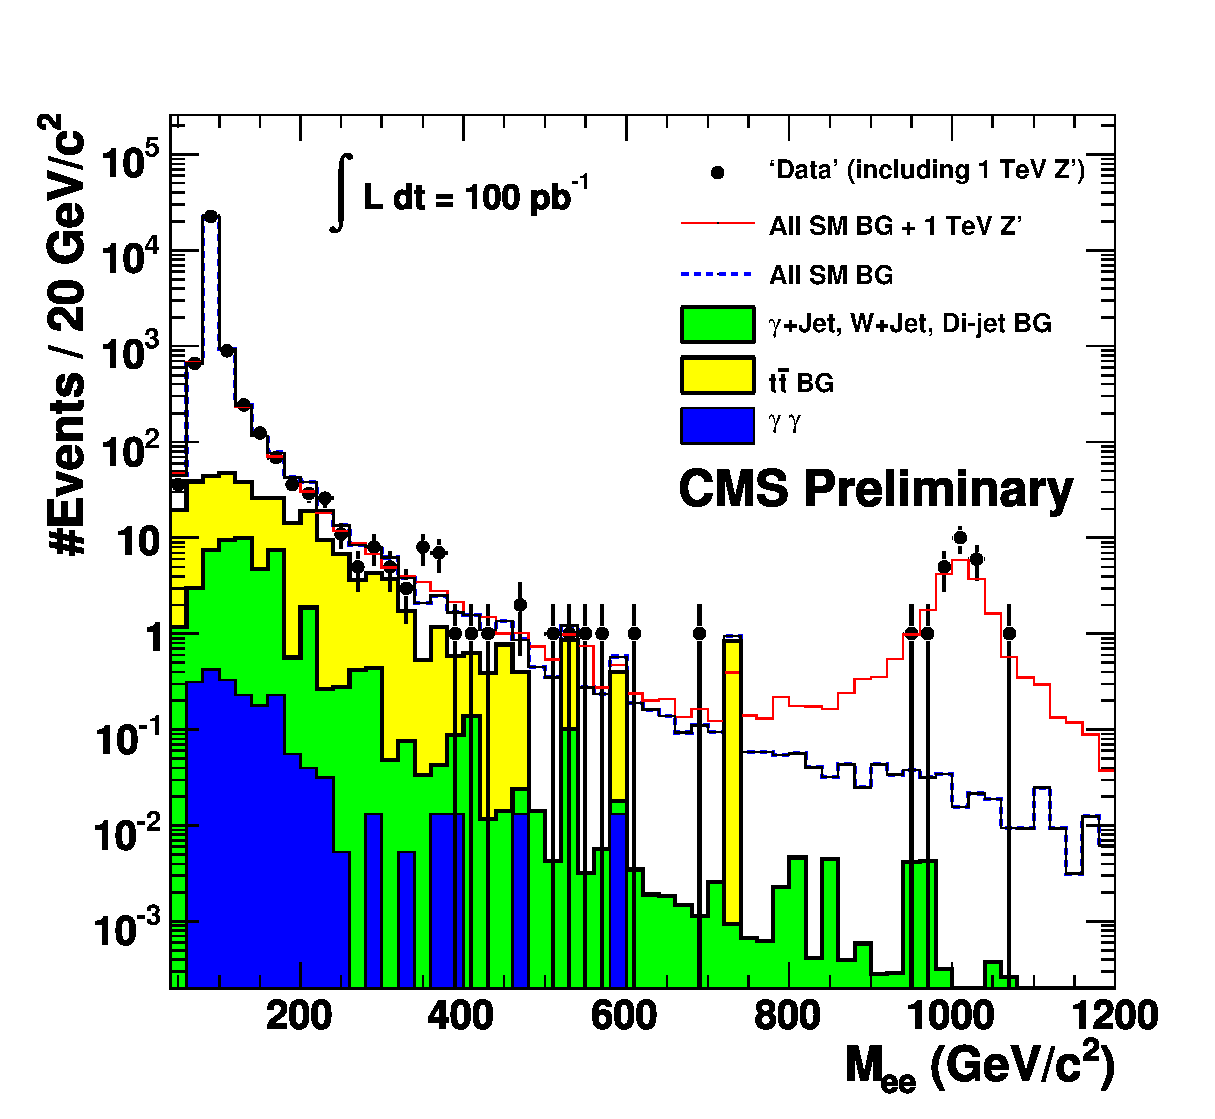
\includegraphics[width=0.45\textwidth]{st_mass_all_withZPrime_ALLTOPO.eps}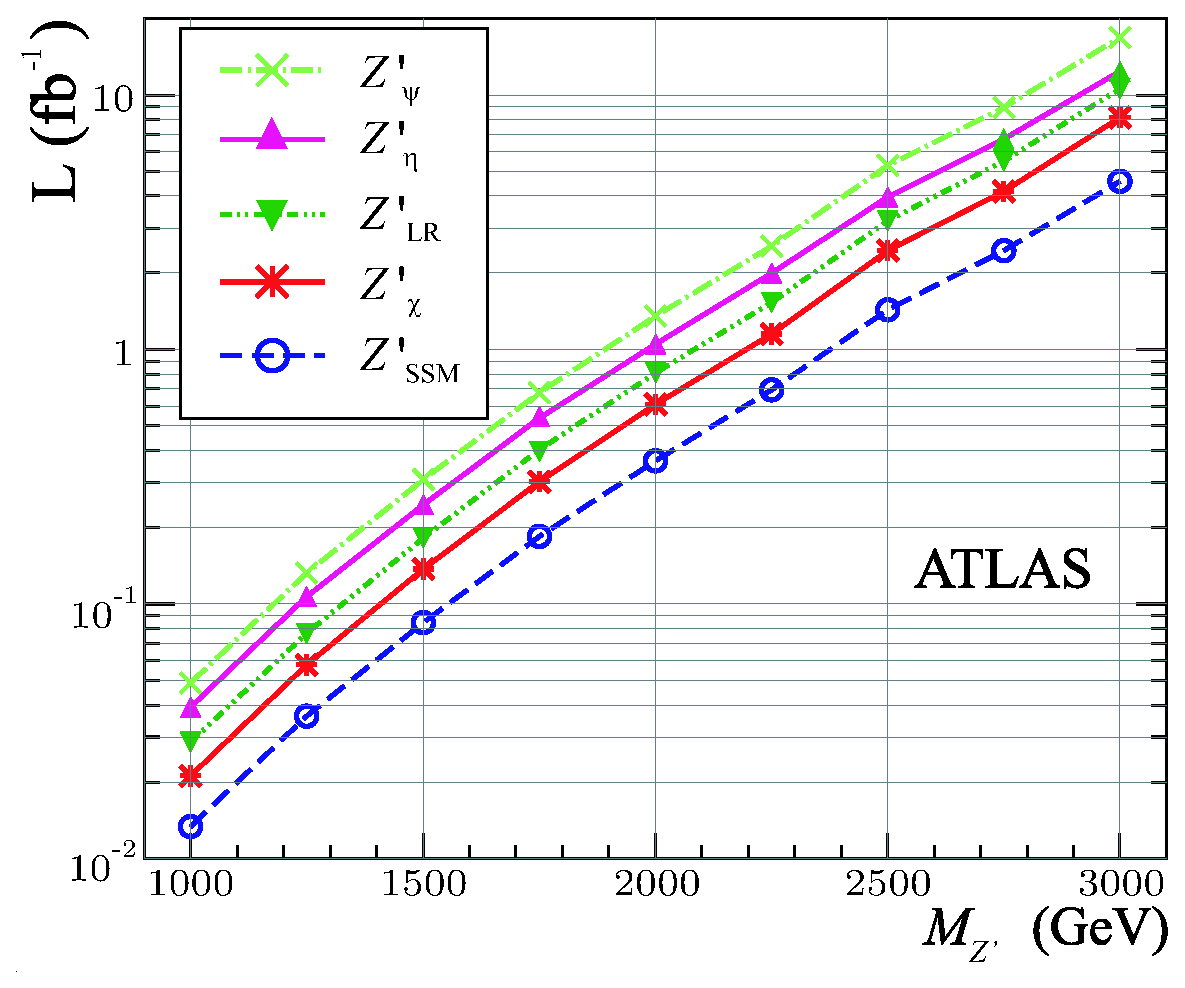
\includegraphics[width=0.45\textwidth]{fig9L.eps}
\caption{Left: di-electron invariant mass spectrum for a 
100~pb$^{-1}$ pseudo-experiment including a signal from 
$Z' \rightarrow ee$ with mass of 1~TeV/$c^2$, 
compared to SM background estimates. Right: integrated 
luminosity needed for a $5\sigma$ discovery of $Z' \rightarrow ee$
as a function of the $Z'$ mass for various benchmark models. Only 
statistical uncertainties are included. 
Effect of systematic uncertainties is less than 20\% in the $Z'$ mass
range investigated.}
\label{fig:MeeAndZPrimeDisc}
\end{figure}

\section{Di-jet channel} \label{dijet}
%The LHC is a parton-parton collider in a previously 
%unexplored energy region. If new parton-parton resonances 
%exist then the LHC will produce them copiously. 
%These resonances should also decay to partons giving two jets in the final state. 
%Therefore the experimental motivation to search for di-jet 
%resonances is intuitively obvious. 
%In addition several theoretical models supports the 
%search of new physics in the di-jet channel (FIXME - ADD REFERENCE). 
%Even if the LHC energy is not sufficient 
Several theoretical models predict the existence of new 
high mass resonances decaying in two 
jets~\cite{Baur:1989kv,Bagger:1987fz,Angelopoulos:1986uq}.
Even if the energy of the LHC is not sufficient to directly produce 
these particles, the new physics might still appear as 
a quark contact interaction~\cite{Eichten:1983hw}, 
and the LHC experiments should 
be able to identify its signals by looking at di-jet events.

%Several experimental approaches have been considered by the 
%ATLAS~\footnote{Results from ATLAS analysis were not yet public at the time 
%of the conference, and therefore not included in this paper.} 
%and CMS (FIXME - ADD REFERENCE) analyses to identify new physics 
%in the di-jet channel, including the study of the jet 
%$p_{T}$ spectrum, di-jet mass, and di-jet ratio.
We discuss here the CMS analysis~\cite{DIJETSNOTE}~\footnote{Results 
from ATLAS analysis were not yet public at the time 
of the conference, and therefore not included in this paper.}
of the di-jet ratio, used to identify the presence of contact interactions. 
The most sensitive search for contact interactions at the Tevatron 
gives an exclusion on the contact interaction scale 
of $\Lambda^{+} < 2.4$~TeV~\cite{Abbott:1998wh}.  

The di-jet ratio is a jet angular variable used to 
discriminate between the new physics and QCD multi-jet events, 
that are the dominant SM background in the di-jet channel. The di-jet ratio is 
defined as $N\mbox{(}|\eta|<0.7\mbox{)}~/~N\mbox{(}0.7<|\eta|< 1.3 \mbox{)}$, 
where $N$ is the number of di-jet events with both jets satisfying the 
pseudo-rapidity requirements in parenthesis. 
Figure~\ref{fig:DiJetRatioAndLQMej} (Left) shows the sensitivity of this 
measurements to contact interactions for different values of $\Lambda^{+}$. 
With 100~pb$^{-1}$ of data, contact interaction with
$\Lambda^{+} < 6.8$~TeV can be discovered, which is well above the 
current Tevatron limits.
 
\begin{figure}[htbp] 
\centering
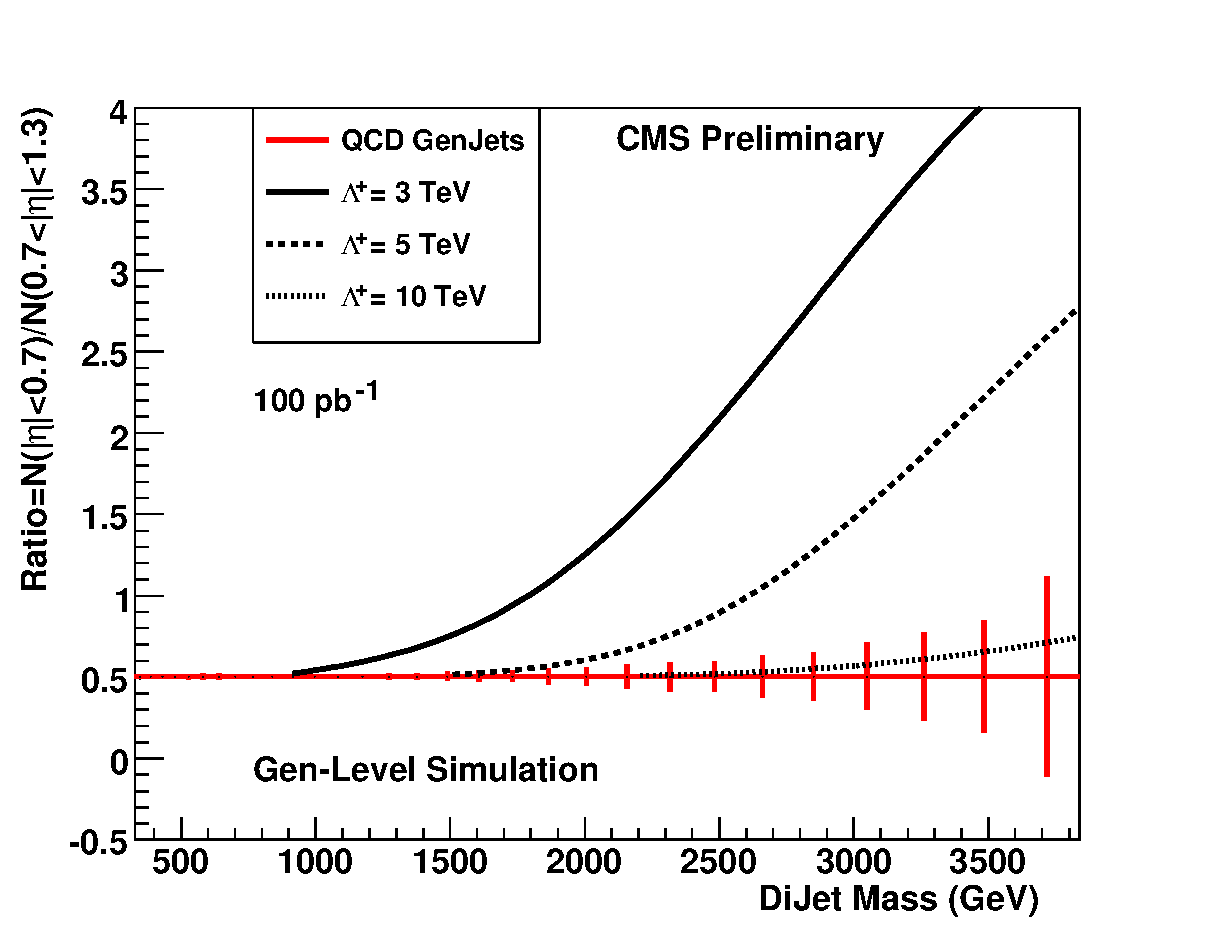
\includegraphics[width=0.45\textwidth]{DiJetRatio100pbOptFix.eps}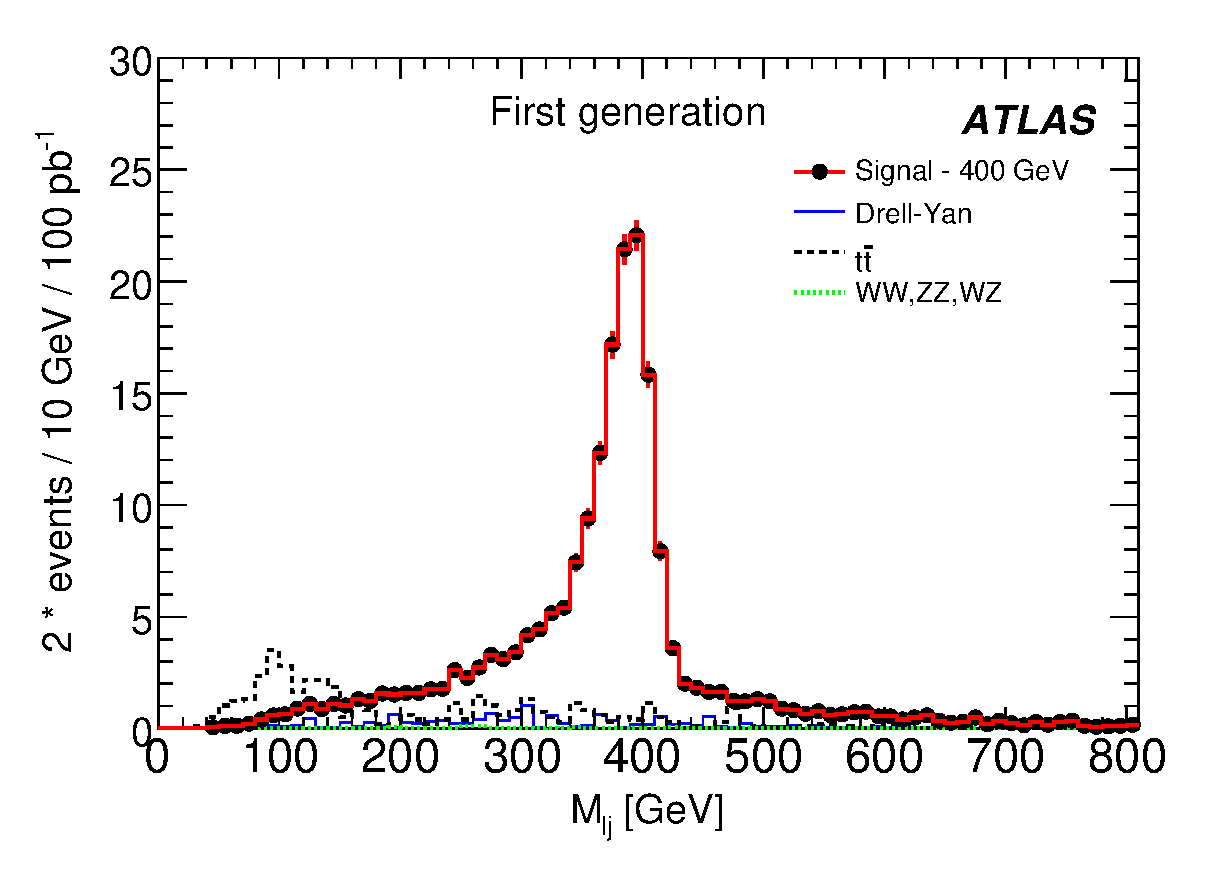
\includegraphics[width=0.45\textwidth]{Mejfig5R.eps}  
\caption{Left: Di-jet ratio as a function of di-jet mass in presence of 
contact interactions at different energy scales $\Lambda^{+}$, 
and for QCD multi-jet background. 
For QCD multi-jet events, the di-jet ratio is almost flat at 0.5. 
In presence of contact interactions, the two 
leading jets are expected to be more central than in QCD multi-jet events, 
thus producing a deviation in the di-jet ratio at high di-jet mass values.
Statistical uncertainties on background estimate are reported.  
Systematics uncertainties, mostly due to jet energy scale, are expected to be small, 
since significantly reduced in the ratio.
Right: Reconstructed electron-jet invariant mass for the signal 
($LQ$ mass of 400~GeV/$c^2$) and the (small) SM background, 
with 100~pb$^{-1}$ of data. If $LQ$s are produced at LHC, 
such striking signature will not be missed.}
\label{fig:DiJetRatioAndLQMej}
\end{figure}

\section{Lepton-jet channel} \label{leptonjet}
Some extensions of the SM predict that new physics would manifest itself in 
final states with high transverse momentum leptons and jets.
For example, the experimentally observed symmetry between 
leptons and quarks has motivated the search for leptoquarks ($LQ$), 
hypothetical bosons carrying both quark and lepton quantum numbers 
that decays in a lepton and a quark~\cite{Acosta:1999ws}.
The lepton-jet invariant mass is a powerful tool to identify the production 
of $LQ$s, as shown in Figure~\ref{fig:DiJetRatioAndLQMej} (Right). 
The ATLAS analysis~\footnote{Results from CMS analysis were not yet public at the time 
of the conference, and therefore not included in this paper.} 
shows that the pair production of scalar $LQ$s, with a branching fraction of 100\% 
in charged electron (or muon) and light quark, can be discovered up to $LQ$ 
mass of about 570~GeV/$c^2$ with 100~pb$^{-1}$ of data~\cite{LQATLAS}. 
The current limit from Tevatron is 256~GeV/$c^2$~\cite{Abazov:2004mk}.

\section{Heavy long-lived charged particles} \label{HSCP}
Some models of new physics 
predicts the existence of exotic particles that are 
heavy (mass of hundreds of ~GeV/$c^2$), long-lived
(enough to decay outside of the detector) and charged~\cite{Fairbairn:2006gg}. 
In the detector, such particles looks like 
minimum ionizing particles, but, differently from the 
relativistic muons, they are slow ($\beta=E/m<1$). 
Standard muon triggers are inefficient for these exotic particles, 
since they arrive late to the muon chambers~\footnote{See details 
in Massimiliano Chiorboli's talk during the conference}. 
Long-lived exotic particles of hadronic nature (such as gluinos or stops) 
can experience also the phenomena of ``charge flipping'' when interacting 
in the calorimeter, thus further complicating their online selection.

Two offline methods are used by the 
CMS analysis to measure their $\beta$~\cite{HSCP}:
$\beta_{{\rm DT}}$ is measured from the time delay arrival of the particle
at the muon chambers~\footnote{ATLAS performed studies to measure 
the value of $\beta$ directly at the level 2 of the online 
trigger system~\cite{Aad:2009wy}}, while $\beta_{{\rm Tk}}$ 
is obtained from the $dE/dx$ measured in the silicon tracker. 
Figure~\ref{fig:HSCPSigBkgPlots} shows the correlation between 
the two $\beta$ measurements for signal (Left) 
and background (Right) events. The analysis results show that 
gluino, stop, and GMSB $\tilde{\tau}$  with mass of about 
1~TeV/$c^2$, 700~GeV/$c^2$, and 200~GeV/$c^2$, 
respectively, can be discovered with 100~pb$^{-1}$ of data.

\begin{figure}[htbp] 
\centering
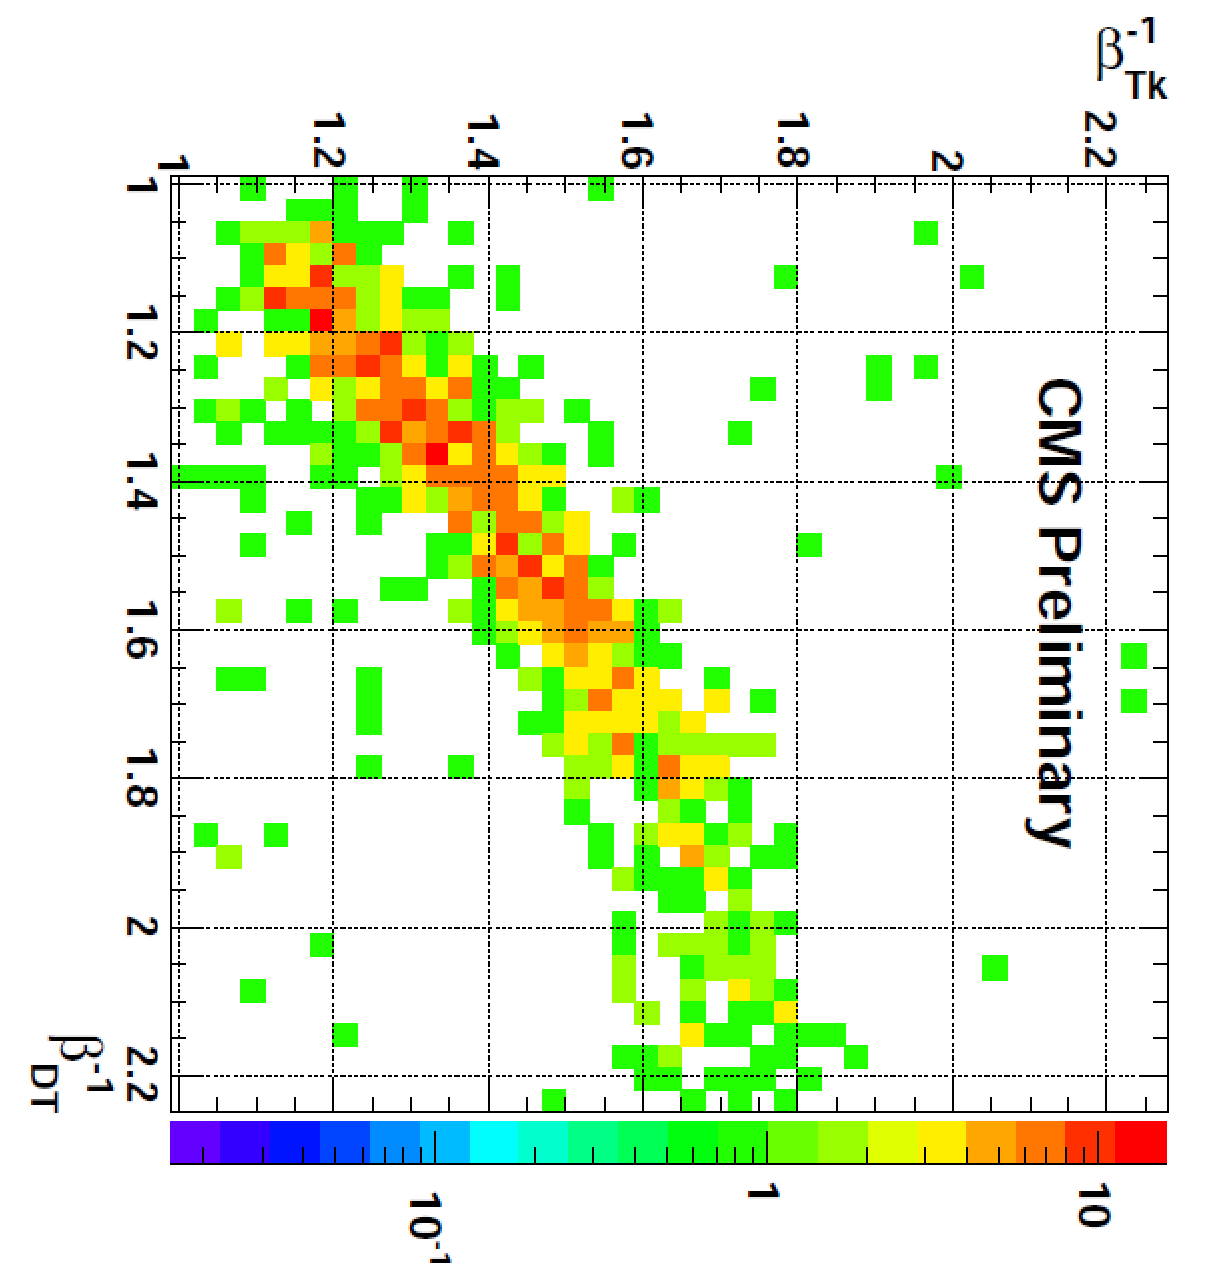
\includegraphics[angle=90,width=0.38\textwidth]{betaHSCPSig.eps}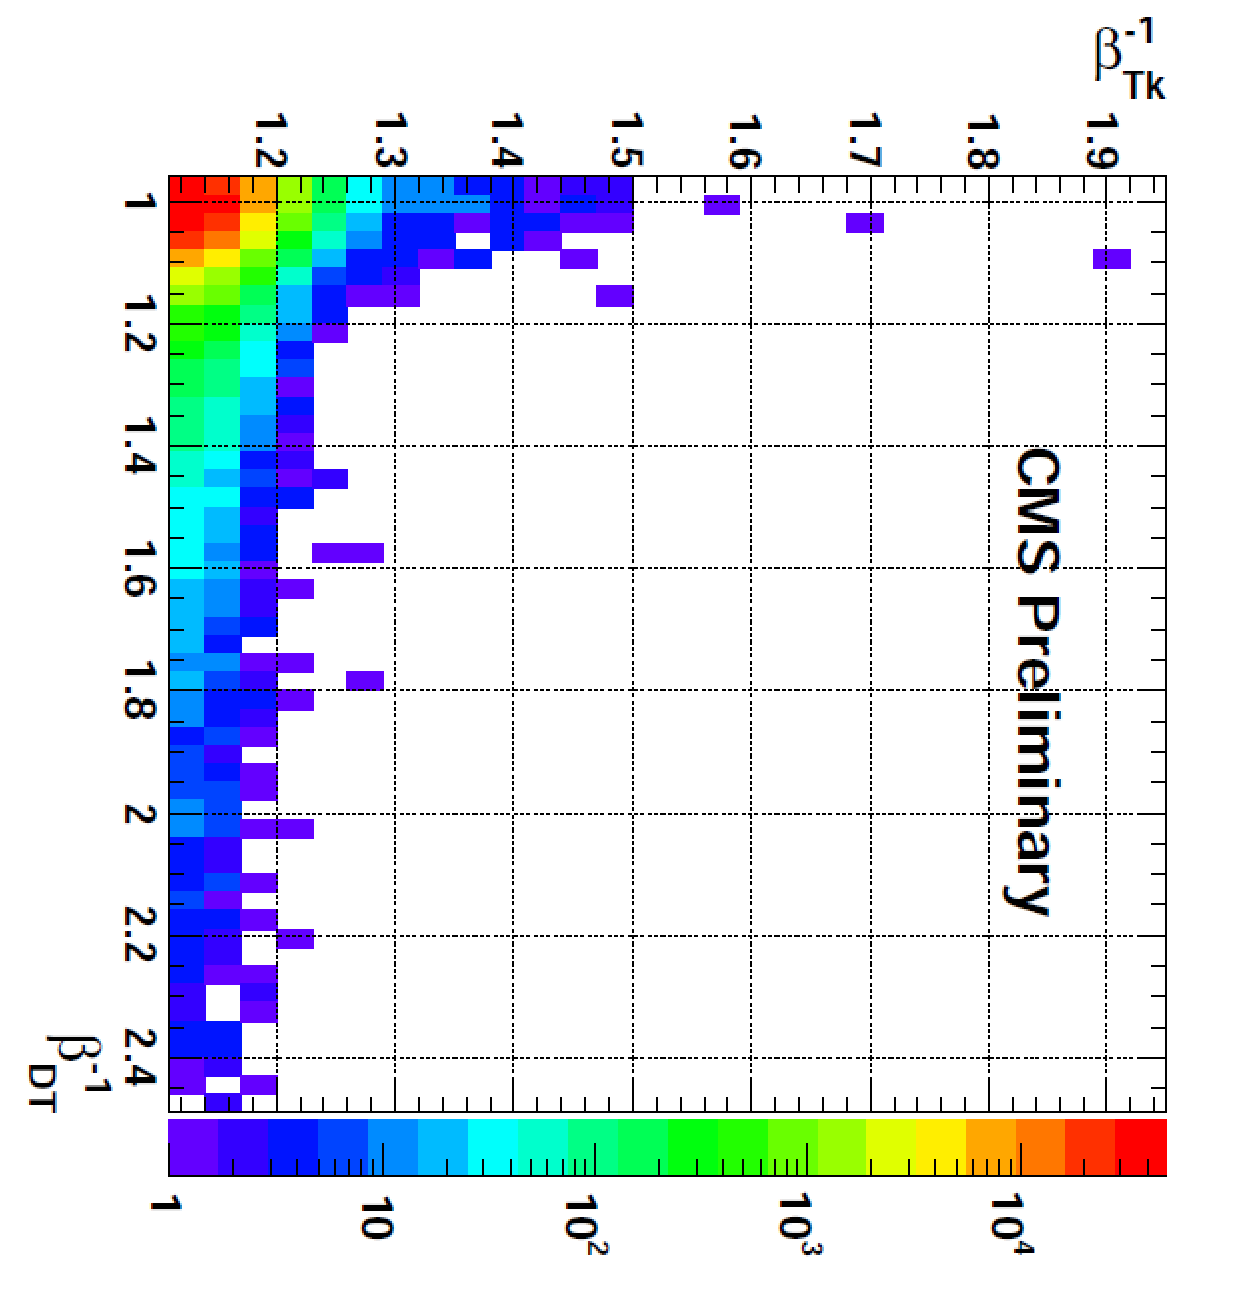
\includegraphics[angle=90,width=0.38\textwidth]{betaHSCPBkg.eps}  
\caption{Distribution of $\beta_{{\rm Tk}}^{-1}$ {\it vs} $\beta_{{\rm DT}}^{-1}$  
for signal (stop with mass of 500~GeV/$c^2$) and for SM background (right), 
for 100~pb$^{-1}$ of data. Despite of the large tails in the background distribution due 
to detector resolution, the signal correlation between the two independent 
$\beta$ measurements allows to define a region of the plane where signal efficiency is 
relatively large and background is almost negligible.}
\label{fig:HSCPSigBkgPlots}
\end{figure}

\section{Conclusion} \label{Conclusion}
Four benchmark analyses has been presented to give an
overview of the Exotica searches in ATLAS and CMS 
experiments at the LHC. The results shown have been obtained with 
MC simulation, assuming 100~pb$^{-1}$ of data and proton-proton collisions
at $\sqrt{s} = 14$~TeV, which is the design energy of the LHC.

Few months before the conference, it has been officially announced 
that the first LHC physics run will be taken at a lower energy 
($\sqrt{s} = 10$~TeV) than the machine design. Preliminary 
studies, performed by the ATLAS and CMS collaborations, 
have shown that the impact of the lower energy is not dramatic for the 
discovery potential of the experiments. In absence of signal observed,
ATLAS and CMS could set, already with the first 100~pb$^{-1}$ of data, 
new constrains on the models of new physics,  significantly more stringent 
than the current Tevatron reach. The updated results,
for the 10 TeV scenario, of the analyses presented here 
(and of many other searches not covered in this short overview) 
will be disclosed by ATLAS and CMS collaborations 
in the next months.

\section{Acknowledgments}
The author wishes to thank the conveners of the New Physics 
section of the conference for their kind invitation. 
He also wishes to thank Maurizio Biasini, Tulika Bose, Giacomo Bruno, Albert De Roeck, Robert Harris, 
Greg Landsberg, Ernesto Migliore, Shahram Rahatlou, Eduardo Ros, Pierre Savard and Claire 
Shepherd-Themistocleous  for the useful discussions and suggestions.

\bibliographystyle{cms-tdr}
\bibliography{references}

%\begin{thebibliography}{0}
%%%%%%%
%%%%%%%
%\bibitem{ref:apo} \BY{Boccaccio~G. \atque de~Cam\~oes~L.}
%  \IN{Phys. Rev. A}{13}{1999}{12};
%  \SAME{69}{999}{1666}.
%\bibitem{ref:pul} \BY{Pulci~L.}
%  preprint INFN 8181.
%\end{thebibliography}

\end{document}

